\clearpage
\title{Problem 4.4}
\author{}
\date{}
\maketitle

\section*{Problem Description}
Write a program to read one of the HEX digits A-F, and display it on the next line in decimal.

\section*{Process}
\subsection*{Code:}

\begin{multicols}{2}{|}
    \begin{minted}[linenos,breaklines,breakanywhere]{nasm}
DATA SEGMENT
    CR EQU 0DH
    LF EQU 0AH
    MSG1 DB CR, LF, "Enter the HEX number : $"
    MSG2 DB CR, LF, "In decimal: 1$"
    NUM DB ?
    DEC_NUM DB ?
DATA ENDS 

CODE SEGMENT
    ASSUME CS:CODE, DS DATA
    
START:
    MOV AX, DATA
    MOV DS, AX
    
    LEA DX, MSG1
    MOV AH, 9
    INT 21H
    
    MOV AH, 1
    INT 21H
    MOV NUM, AL
    
    SUB NUM, 11H
    
    LEA DX, MSG2
    MOV AH, 9
    INT 21H
    
    MOV DL, NUM
    
    MOV AH, 02H
    INT 21H
    
    MOV AH, 4CH
    INT 21H
CODE ENDS
END START
\end{minted}
\end{multicols}

\subsection*{Output}
\begin{center}
    \centering
    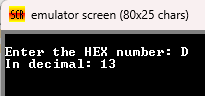
\includegraphics[width = .4\textwidth]{4.png}
    \captionof{figure}{Converting HEX (A-F) to Decimal}
\end{center}
